%% -*- latex -*-
\documentclass[a4paper]{article}
\usepackage{times,epsf,amsmath,amssymb}
\usepackage{setspace}
\usepackage{pgf}
\usepackage{tikz}
\usetikzlibrary{decorations}
\usetikzlibrary{backgrounds}
\usetikzlibrary{patterns}
\usetikzlibrary{snakes}
\usetikzlibrary{shapes}
\usetikzlibrary{arrows}

\usepackage{xcolor}
\usepackage{hyperref}
\definecolor{DarkRed}{RGB}{100,0,0}
\hypersetup{urlcolor=DarkRed,urlbordercolor=DarkRed}

\usepackage{minted}
\usepackage[skins]{tcolorbox}
%\usepackage{todonotes}
%\usepackage{draftwatermark}
\usepackage[british]{babel}

\usepackage[scale={0.7,0.8}]{geometry}
\begin{document}

\title{University of Northumbria\\
CM0506 -- Small Embedded Systems\\
        ---\\
       Assignment 1: Pong}
\date{Semester 1, 2016}
\author{M J Brockway and A J Moon}

\maketitle

\section{Introduction}
This assignment is as follows: 
\begin{enumerate}
\item an exercise in programming the ARM microprocessor and associated
  peripherals in C to implement a simple game using digial and
  analogue inputs and the LCD screen.   This program will be assessed on:
  \begin{itemize} \setlength \itemsep{0em}
  \item how well it works - your code will be tested;
  \item the structure, style and layout of the code;
  \end{itemize}

  % \item a short report on relevant aspects of embedded system
  %   programming, around 7-8 pages (about 4500 words) in length.

  %   There is no fixed penalty for exceeding this limit, but a
  %   verbose, poorly constructed report containing irrelevant
  %   material will not attract a good mark.
\end{enumerate}

\subsection{Assessment and Deadlines}
The mark for this assignment will contribute one-third to the final mark
for this Module.  

An indication of how marks are to be allocated is given in
sections~\ref{progMrkg}.  Important dates for this
assignment are:
\begin{itemize}
\item Assignment is set in week 4 (10 October)
\item Working programs to be demonstrated in the Assessment Periods
  Tuesday 3 January 2017 to Friday 13 January 2017.  A timetable of
  demonstrations will be published in advance of the demonstration
  week.
\item Submission is {\bf electronic}, via the e-Learning Portal, by
  Tuseday 3 January.  
\item Marks and feedback will be available about three weeks
  thereafter, by e-mail plus meeting if desired.
\end{itemize}

This gives you 8 weeks (excluding the vacation period) to complete the
assignment.  Time will also be allowed within the last few practical
sessions to work on the assignment and obtain guidance from your
tutor.

\paragraph{Note}  There will be a checkpoint in the mark-scheme on
Blackboard to tick off stages in the process.  This will allow me to
keep track of you all, and check that the submission mechanisms work.

\clearpage
\subsection{Learning Outcomes Addressed by this Assignment}
\begin{enumerate}
\item Demonstrate an appreciation of the architecture of a range of
  different microprocessors/microcontrollers and display a detailed
  understanding of a particular device.
\item Use a variety of software development tools to produce, test and
  debug software for small embedded systems in C and assembly language
  (partially)
\item Describe and apply best practice in software development for the
  use of a variety of system and user peripherals associated with a
  modern microcontroller.
\item  Characterise and use specifications of typical
  transducers, actuators and network controllers to interface them to
  a microcontroller and develop device driver software to make such
  devices conveniently available for use by an application developer.
\end{enumerate}


\subsection{Academic Misconduct}
  Please
read the University Guidelines on Academic Misconduct.

\subsection{Structure of this Document}
The sections of this document are organised as follows.
\begin{description}
\item[Section~\ref{progSpec}] describes Part A of the assignment; it provides
the background to the problem, a specification of the control system
in section~\ref{reqts}.  Notes on your implementation and a suggested
algorithm for the game is presented in section~\ref{implementation}.
The stages of the assignment are outlined in section~\ref{stages} and
section~\ref{technical} offers some technical hints.
\item[Section~\ref{progMrkg}] gives the breakdown of marks.

\end{description}

\clearpage
\section{Program: The Pong Game}\label{progSpec}
The game area is a rectangular ``court". A small coloured ball moves
inside the court, bouncing off the side walls and the top wall at the
same angle as it struck.  The ball goes out of play when it reaches
the bottom wall of the court but above this is a small bat which can
be moved from side to side by the player; the ball may be bounced off
this back up into the court and remain in play.

The player earns points by keeping the ball in play as long as
possible; the scoring rate increases as a ball remains in play.
 
% The game is called \emph{Tilt}Pong because the player will control
% the side-to-side movement of the bat using the accelerometer,
% tilting the ARM board.

  
\subsection{Requirements} \label{reqts}

\subsubsection{The playing area}
The court is a rectangle within the display area of the LCD.  Most of
the display area of the LCD is devoted to the game display and is
rendered in white.  A top border displays the score and number of
remaining balls, as indicated here:

\begin{center}
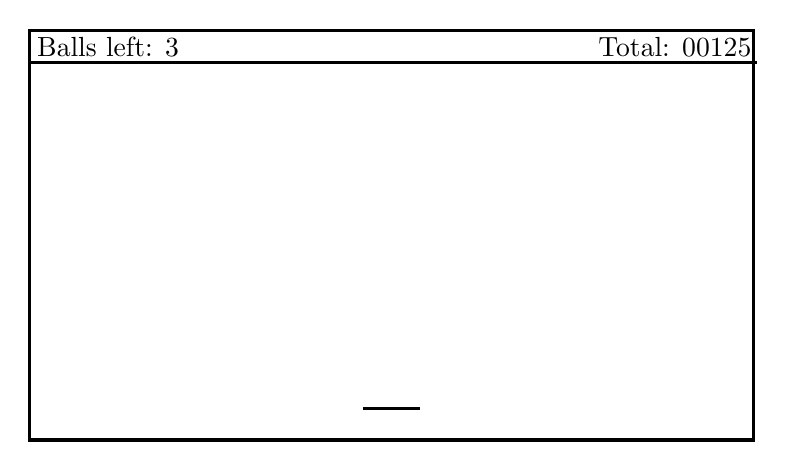
\begin{tikzpicture}[scale=0.04]
  \filldraw[fill=white] (0,0) rectangle (230,130);
  \draw[black,very thick] (0,0) rectangle (230,130);
  \draw[black,very thick] (0,120) -- (231,120);
  \draw[black] (25,125) node {Balls left: 3};
  \draw[black] (205,125) node {Total: 00125};
  \draw[black, very thick] (106,10) -- (124,10); 
\end{tikzpicture}
\end{center}

\subsubsection{The bat}
This is black, 40 pixels wide and 4 pixels high. Initially it is a
random distance across the court and 10 pixels above the bottom. Its
sideways movement is controlled by the joystick or by tilting the ARM
board; it does not move vertically.

\subsubsection{The ball}
The ball is to be rendered as a filled blue circle 10 pixels in
diameter. It moves within the court, bouncing off the side and top
walls and the bat.

\begin{center}
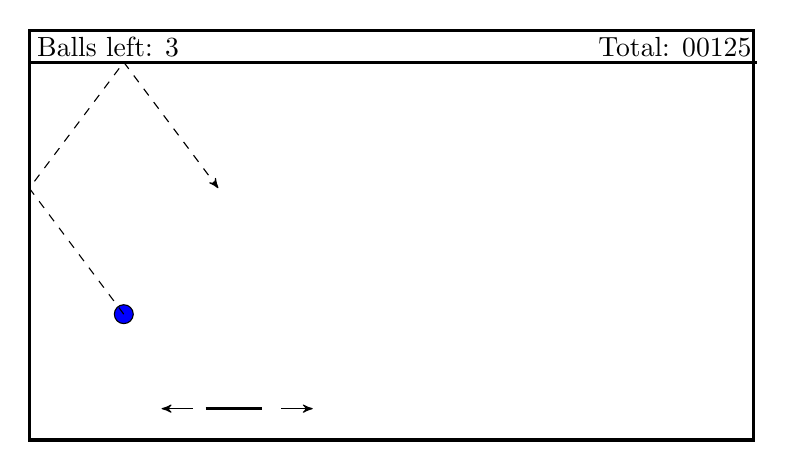
\begin{tikzpicture}[scale=0.04]
  \filldraw[fill=white] (0,0) rectangle (230,130);
  \draw[black,very thick] (0,0) rectangle (230,130);
  \draw[black,very thick] (0,120) -- (231,120);
  \draw[black] (25,125) node {Balls left: 3};
  \draw[black] (205,125) node {Total: 00125};
  \draw[black, very thick] (56,10) -- (74,10); 
  \draw[black, ->, >=stealth'] (80,10) -- (90,10);
  \draw[black, <-, >=stealth'] (42,10) -- (52,10);

  \filldraw[fill=blue] (30,40) circle (3);
  \draw[black, dashed] (30,40) -- (0,80) -- (30,120);
  \draw[black, dashed, ->, >=stealth'] (30,120) -- (60,80);
\end{tikzpicture}
\end{center}

The bat movement must be controlled to catch and return the ball
before it goes out of play.

The game is started by a press on the joystick CENTRE: a new ball
starts moving down the court at a random speed and in a random
direction.

If it strikes the side walls or bat, the ball bounces spinlessly --
the angle of reflection equals the angle of incidence. (The easiest
way of implementing this is to have one of the velocity components
change sign while the other stays the same.)

If the ball is caught by the bat it bounces in the same fashion, up
toward the top of the court.  Otherwise it goes out of play at the
bottom.

After a new ball the player earns a point each time the ball reaches
the top of the court.  After 5 such ``returns" of this ball the
scoring rate increases to 2 points balls for each return; after 10
returns, 3 points per return and so on. As long as the ball remains in
play the scoring rate grows by a point every 5 successful returns.

When a ball goes ``out" the player can summon a new ball with another
press of joystick CENTRE but the scoring rate is reset to 1. The score
for ``This ball" is reset to 0 but the ``Total" score remains.

The game is over after 5 new balls. Joystick CENTRE will start a new
game but \emph{both} scores are reset to 0.

\medskip

\begin{tcolorbox}
  \emph{Successful software development to this stage will provide a
    basic pass of 50\% for the run-time assessment.}
\end{tcolorbox}
\medskip

\clearpage
\subsubsection{An Obstacle}
A line of random length between 40 and 200 pixels (shown two pixels
thick in green) is positioned somewhere in the top half of the playing
area. The obstacle behaves like a wall: the ball bounces spinlessly
off it. (But without earning points -- only the top wall of the court
counts for this.)

\begin{center}
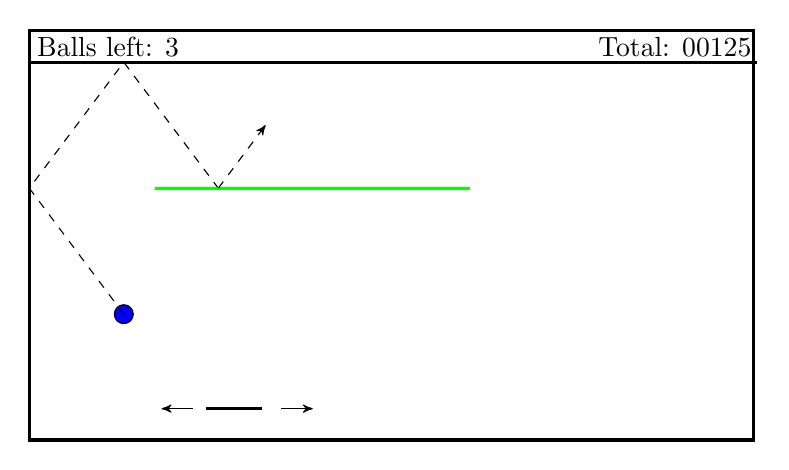
\begin{tikzpicture}[scale=0.04]
  \filldraw[fill=white] (0,0) rectangle (230,130);
  \draw[black,very thick] (0,0) rectangle (230,130);
  \draw[black,very thick] (0,120) -- (231,120);
  \draw[black] (25,125) node {Balls left: 3};
  \draw[black] (205,125) node {Total: 00125};
  \draw[black, very thick] (56,10) -- (74,10); 
  \draw[black, ->, >=stealth'] (80,10) -- (90,10);
  \draw[black, <-, >=stealth'] (42,10) -- (52,10);

  \filldraw[fill=blue] (30,40) circle (3);
  \draw[black, dashed] (30,40) -- (0,80) -- (30,120) -- (60,80);

  \draw[green, very thick] (40,80) -- (140,80);
  \draw[black, dashed, ->, >=stealth'] (60,80) -- (75,100);
\end{tikzpicture}
\end{center}


\subsubsection{Magic Time}
A ``magic time'' period occures at random intervals of between 5 and
10 seconds - i.e, between 5 and 10 seconds after the last ``magic
time" period, and lasts for a random duration of 2 to 10
seconds. During ``magic time" the ball is displayed red and the
scoring rate is double.

\begin{center}
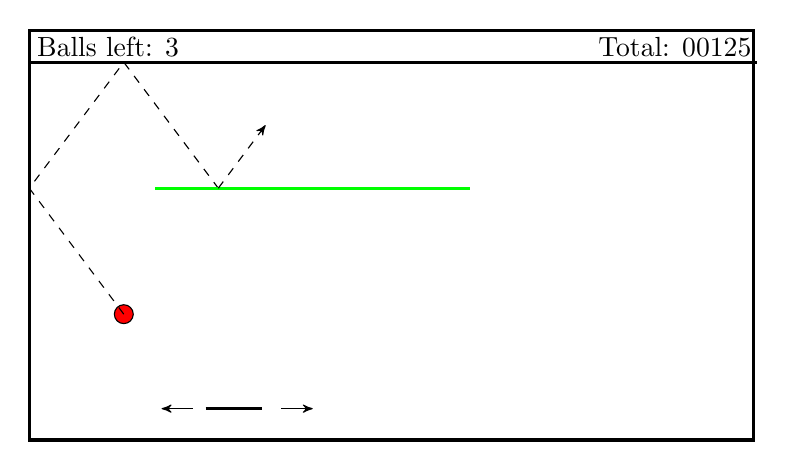
\begin{tikzpicture}[scale=0.04]
  \filldraw[fill=white] (0,0) rectangle (230,130);
  \draw[black,very thick] (0,0) rectangle (230,130);
  \draw[black,very thick] (0,120) -- (231,120);
  \draw[black] (25,125) node {Balls left: 3};
  \draw[black] (205,125) node {Total: 00125};
  \draw[black, very thick] (56,10) -- (74,10); 
  \draw[black, ->, >=stealth'] (80,10) -- (90,10);
  \draw[black, <-, >=stealth'] (42,10) -- (52,10);

  \filldraw[fill=red] (30,40) circle (3);
  \draw[black, dashed] (30,40) -- (0,80) -- (30,120) -- (60,80);

  \draw[green, very thick] (40,80) -- (140,80);
  \draw[black, dashed, ->, >=stealth'] (60,80) -- (75,100);
\end{tikzpicture}
\end{center}

\subsubsection{Ball speed}
The speed of the ball may be controlled by adjusting the position of
the potentiometer on the board.  The control should adjust speed from
``very slow'' to ``impossibly fast''.

\subsubsection{Game Controls}
\begin{itemize}
\item The bat is moved by moving the joystick left or right, or by
  tilting the board.  Small changes in board angle should have no
  effect (small, random hand movements should be ignored).
\item The game is started (and restarted) by pressing joystick CENTRE,
  which also delivers a new ball. A game consists of 5 new balls.
\item The potentiometer position controls the speed of the ball.
\end{itemize}

\clearpage
\subsection{Implementation}\label{implementation}
See
{\href{https://classroom.github.com/assignment-invitations/e0d3930cc5cf943bd1c10642b750ac8e}{GitHub
  classroom}
 for a starting point.  Technically it is an invitation to join the
 assignment, and get some initial code.

\subsubsection{Constraints}
Certain aspects of the C implementation must be adhered to and will be
subject to assessment, namely:
\begin{description}
\item [Decomposition] - your solution should show good decomposition
  (place different functionalities or responsibilities in different
  software components) - make good use of functions to encapsulate
  code in a sound engineering fashion.  Your functions should be short
  (no longer than about half a page).  The {\tt main()} function
  should simply call other functions - to initialise the game and play
  the game, for example;
\item [Coherence] - similar tasks, related to each other, are handled
  by particular functions;
\item [Low Coupling] - modification of one subsystem should have
  little impact elsewhere;
\item [Managed Complexity] - your solution should be sufficient and
  complete but no more complex than justified;
\item [Documentation] - ensure that you document your code to the
  correct degree.  This should include headings on each function - the
  purpose, algorithm (if appropriate), and comments before each
  section if this aids clarity.  Statement comments will only rarely
  be necessary if your coding style is clear.
\item [Global data] - avoid global data declarations - make full use
  of parameter passing and return values for function calls.  Some use
  of global data cannot avoided (shared data between the interrupt
  service function and the main code, for example).  However, this
  must be reduced to the minimum and documented;
\item [Identifiers] - choose identifiers with care and be consistent
  in their naming;
\item [Literal Values] - avoid literal constants for such things as
  boundary limits, the position of the obstacle, etc, like this:
\begin{minted}{c}
     if ( ball.x > 76 )
        ...
\end{minted}
  use \mintinline{c}{#define} or \mintinline{c}{const} or \mintinline{c}{enum} to declare such
  values and make them very visible;
\item [Use of a Timer Interrupt] - a timer interrupt service {\bf
    must} be used to manage the periodic occurrence and end of ``magic
  time".  A timer interrupt period of 1 second is appropriate. Pay
  particular attention to the safety of data access by both the
  interrupt service and the main-line code, and \emph{do not} give the
  interrupt service routine too much to do. Setting certain status
  variables should suffice here.
\end{description}


\subsubsection{Data Structures}
You may implement any data structures you wish - for instance, for
storing bat, ball states.  Your selection of appropriate data
structures \emph{will} be assessed.  For example, you might use {\it
  struct} records to hold related data - ball coordinates, velocity
components, etc.

\clearpage
\subsubsection{Algorithms and Data Structures}
The following (incomplete) algorithm is suggested as a starting point
for the basic game:

\begin{minted}{c}
   initialiseDevices();
   remainingBalls = initialiseGame();

   while ( remainingBalls > 0 ) {

      waitForStart();

      ballInPlay= 1;
      batPos = initialiseBatBall( ball );
      renderBall( ball );
      updateBall( ball );
      renderBat(batPos);

      while ( ballInPlay ) {
         renderBall(ball);
         updateBall( ball );

         batMovement = ReadBoardAngle();
         batPos = adjustBat ( batMovement );
         renderBat(batPos);
         ballInPlay = testBottom( ball );
         delay();
      }
   }
 \end{minted}


Your \mintinline{c}{main()} function should be no more complex than this for the
basic game.  Note the use of functions to encapsulate low-level
detail.

For managing the ball, you might consider a record type as below. 

Rendering the ball consists in drawing a filled circle of appropriate
colour and radius at $(x, y)$.

Updating the ball might just be adding \mintinline{c}{vx},
\mintinline{c}{vy} (or a multiple?) to \mintinline{c}{x},
\mintinline{c}{y} and then adjusting \texttt{vx} or \texttt{vy}
 appropriately if a
collision is detected. A collision with a verticle wall will mean
\texttt{vx = -vx} and with a horizontal wall (obstacle, top of court,
bat) will mean \texttt{vy = -vy}. Do not forget updating the score if
a collision with top is detected -- define a subroutine for
this. Think how you will detect bounces.

\begin{minted}{c}
   typedef struct Ball {
      int x, y; //position coordinates
      int vx, vy; //velocity components
      int colour;
   } ball_t;

  ball_t ball;
\end{minted}

To initialise the bat and the ball you might set the bat position
initially to be half way across the court. The ball should initially
be near the top of the court, a random amount across and random
velocity components causing the ball to head down the court. The
x-velocity should be less than the y-velocity. You will need to
experiment with random values -- see Technical Tips section below.

\clearpage
\subsection{Work Plan}\label{stages}
A skeleton starting point should be available through the
\href{https://classroom.github.com/assignment-invitations/e0d3930cc5cf943bd1c10642b750ac8e}%
{GitHub classroom}, and also through a link on Blackboard

If you are struggling, it will be better to provide a partial solution
which works properly than an unsuccessful attempt at a complete
solution.  Similarly, it will be better (and easier) to provide a
partial solution that is properly documented, than a complete solution
without any documentation, as the later stages of the assignment are
more difficult than the early stages.  You are recommended to complete
the work in phases as follows:

\begin{enumerate}
\item Initialise the devices you require, buttons, LCD, accelerometer,
  but do this in an initialisation function called from main. Write a
  function to initialise the score, number of balls and the
  display. Test this by calling it from {\tt main()}.

\item Design a data structure for the ball coordinates and velocity
  components.  Should the colour be included? Write functions for
  initialising, rendering and updating the ball and bat. Test this
  part with a suitably simplified main loop.

\item Introduce a function to poll the joystick CENTRE and wait until
  it is pressed before starting a game or ball.

\item Write a function to move the bat in steps left or right in
  response to the joystick.  Then extend this to move the bat in
  response to tilts detected by the accelerometer.  Only the X value
  need be used for this. There should be no response to very small
  accelerometer readings: you will need to experiment to determine
  right cutoff value.

\item Write a function to update the score when a collision with the
  top of the court is detected.

\item Write a function to detect when the ball has gone out of play.

  \emph{Successful development up to this stage will give you a basic
    pass (50\%) with the code run-time assessment.}

\item Introduce the obstacle in the top half of the court.  Extend the
  collision function to detect obstacle collisions.

\item Introduce a timer interrupt to manage ``magic time".  It is
  suggested that the interrupt service simply sets/clears flag
  variables to manage start and duration. The main-line code can
  access these (globals) to manage the consequent game logic and
  rendering.  Update ball rendering and scoring functions as
  appropriate.

\item Implement any additional functions including the speed control.
\end{enumerate}

\subsection{Technical tips}\label{technical}
\begin{itemize}
\item The standard C function {\tt rand()} returns a random number in
  the range 0 to {\tt RAND\_MAX}, defined in {\tt <stdlib.h>}.  To
  produce a random integer {\tt r} between 0 and {\tt N-1} use
\begin{minted}{c}
    r = rand() % N;
\end{minted}
  Thus \texttt{a + rand()\%(b-a)} gives a random integer between
  \texttt{a} and \texttt{b-1} (assuming \texttt{a < b}).
\item Test each (small) addition to your program with care - do not
  write long sections of code before testing.

\item Save your code using different file versions between major edits
  to allow recovery to an earlier version if disaster strikes!
\end{itemize}

\clearpage
\subsection{Marking scheme}\label{progMrkg}
Marks will be awarded for \emph{functionality} and for \emph{program
  style and structure}:

\begin{description}
\item [Program Functionality, 35\%] is based entirely on how well the
  program works under test.  The software test will be performed with
  you present to allow clarification of possible strange
  behaviour. Marks are broken down as follows:
\begin{itemize}
\item Basic Game (17\%)
  \begin{itemize}
  \item 2\% - Game playing-area display, score and remaining balls
  \item 1\% - Bat rendering
  \item 2\% - Bat moves in response to accelerometer input
  \item 2\% - Ball rendering and movement
  \item 2\% - Initial ball moving down court with random direction,
    speed
  \item 3\% - Bounces off top, sides, bat working
  \item 1\% - Waits for joystick CENTRE before starting
  \item 2\% - Ball going out causes a wait for new game; remaining
    balls value is adjusted
  \item 2\% - Scoring 
  \end{itemize}
\item Advanced Features (18\%)
  \begin{itemize}
  \item 5\% - Obstacle displayed and collision of ball with it
    detected
  \item 5\% - Magic time comes and goes at required intervals
  \item 5\% - Ball and scoring during Magic time, 
  \item 3\% - Game speed adjustable via the potentiometer
  \end{itemize}
\end{itemize}
Partial marks may be awarded for attempted but incomplete (or poorly
implemented) features. You will be asked questions concerning your
solution and your code to confirm your ownership of the work.

\item [Program Style and Structure 15\%] Based on the layout of the
  program, the use of comments and subroutines and the style of
  programming. Adopt a sound engineering approach in developing the
  code to aid the future maintenance of the software.  Particular
  attention should be made to sound decomposition and use of
  functions.  Marks will be awarded as follows (see notes in
  Section~\ref{implementation}):
\begin{itemize}
\item 5\% - Documentation, variable naming, layout and clarity
\item 5\% - Decomposition into functions 
\item 5\% - Use of the timer interrupt to manage ``magic time"
\end{itemize}
Marks will only be awarded here for a program that compiles cleanly
and performs the basic game action. 
% {\bf Include a paper listing of the program.}\todo{Electronic submission, GIT and BB}
\end{description}

\clearpage
\subsection{Submission of code:}  
\begin{quote}
  A little complex, but we are trying something new here.
\end{quote}

\paragraph{Firstly} Sign up for a GitHub account
\textbf{\url{https://github.com}}.  Then you can get the ``Student Developer
Pack''  which gives you tools and private repositories.
See \textbf{\url{https://education.github.com}}

\paragraph{Do use \texttt{git} to keep  your code}.  Using version
control is good practise.  Syncing  keeps a copy safe on GitHub's
servers.

\paragraph{There are 3 actions  in the submission plan}
\begin{enumerate}
\item Submit through blackboard. \\ Submit two items 
  \begin{itemize}
  \item the URL of your repository.
  \item a listing of \emph{your} files (\texttt{.c} and \texttt{.h}),
    just the ones you have written, you don't need to submit libraries
  \end{itemize}
\item Submit through the
  \href{https://classroom.github.com/assignment-invitations/e0d3930cc5cf943bd1c10642b750ac8e}{GitHub
    classroom}.  Accepting the invitation to the assignment should
  make this automatic.  (I hope)
\end{enumerate}
 
\paragraph{A note on listings}  I use a couple of nice Unix tools to
create pdf listings from code.  On my laptop (a windows machine) I use
\href{https://www.cygwin.com/}{Cygwin} to give me a Unix environment.

The commands I use are
\begin{minted}{bash}
a2ps --header="Alun Moon" -1 --output=alun.moon.ps main.c timer.[ch]
ps2pdf alun.moon.ps
\end{minted}

\subparagraph{a2ps} is a nice text to Postscript converter that
pretty-prints C code
\begin{description}
\item[--header] The \texttt{--header} option puts a name at the top of
  the page (include your student id)
\item[-1] The \texttt{-1} option puts the output in portrait, with 1
  column
\item[--output] The output option specifies the file to write the
  Postscript to.  By default \texttt{a2ps} sends its output directly
  to the printer.  Use your name for the file, otherwise I get 130
  files all called \path{code.pdf} or \path{listing.pdf}
\item[files] list the files in the order you want them to appear in
  the listing.
\end{description}

\subparagraph{ps2pdf} converts the Postscript file into PDF.  In the
example it automatically names the output file \path{alun.moon.pdf}

You don't have to use this method to generate the PDF file,
\begin{itemize}
\item You could print-to-pdf from the uVision and then combine the
  pdfs for each file into one
\item Use Word!
\item something else.
\end{itemize}


\end{document}

%% Local Variables:
%% mode: reftex
%% mode: auto-fill
%% mode: flyspell
%% End:


\newpage

\section{Report - Theoretical Aspects of ARM
  Programming}\label{rptSpec}\label{rptMrkg}
You are asked to address some theoretical aspects of your work, as
follows.

\begin{description}
\item [Testing Strategy, 10\%] - What strategy would you adopt to test
  your software?  Do not present test results - simply describe what
  testing procedure you would use at each stage in development to
  raise your confidence that the software would behave as specified.

\item [Interrupt Safety, 10\%] - Although not a safety critical
  application, and malfunction of the game does not present any user
  safety concerns, the use of an interrupt introduces additional data
  integrity and concurrency difficulties.  Describe briefly what
  additional problems are raised by using concurrency (interrupt code
  and main-line code) and what precautions you would take to ensure
  correct operation.

\item [Timing, 10\%] - A feasible way to achieve a suitable time delay
  for the Pong game is ro use a \emph{busy wait}. You have used this
  in lab exercises early in the module. Describe what this is, and
  contrast it with a solution based on \emph{timer interrupts} -- what
  are the relative advantages and disadvantages of each approach?

\item [Input and Output on the ARM, 10\%] - Describe what
  memory-mapped input/output is, and how input and output are set up
  and performed on the ARM board.  Describe in detail how LED1 is
  switched on/off and how a Joystic gesture is captured and reported
  to the the game software. What other things must the device driver
  software do?

\item [Best Practice, 10\%] Discuss the principles of \emph{best
    practice} that should be applied in general and in embedded
{  programming in particular.
\end{description}

% \item [Embedded System, 10\%] Discuss the feature of embedded
%   systems that distiguish them more other types of comuting system.

% \item [ARM Architecture, 10\%] Give a brief overview of the main
%   features of the ARM embedded CPU architecture. What are the major
%   components, and how do they interact?

Your short report should be up to 10 pages in length - around 2 pages
for each section. The resources listed on the module web page will be
useful.


